\documentclass[a4paper,12pt]{article}

\usepackage[utf8]{inputenc}
\usepackage{graphicx}
\usepackage{amsmath}
%\usepackage[english]{babel}
\usepackage{url}
\usepackage{booktabs}
\usepackage[T1]{fontenc}
\usepackage{lmodern}
\usepackage{float}
\usepackage{tocloft}

\usepackage[T1]{fontenc}

\setlength{\parskip}{1em}
\setlength{\parindent}{0pt}

\usepackage{graphicx}
\usepackage{float}

\renewcommand{\figurename}{Slika}

\usepackage{listings}
\usepackage{xcolor}

\lstset{
    language=Python,
    basicstyle=\ttfamily\small,
    keywordstyle=\color{blue},
    commentstyle=\color{gray}\itshape,
    stringstyle=\color{red},
    numbers=left,
    numberstyle=\tiny\color{gray},
    stepnumber=1,
    numbersep=5pt,
    showstringspaces=false,
    breaklines=true,
    frame=single,
}

\renewcommand{\figurename}{Slika}
\renewcommand{\tablename}{Tabela}

\begin{document}

\begin{titlepage}
    \centering
	\begin{figure}[htbp]
    	\centering
    	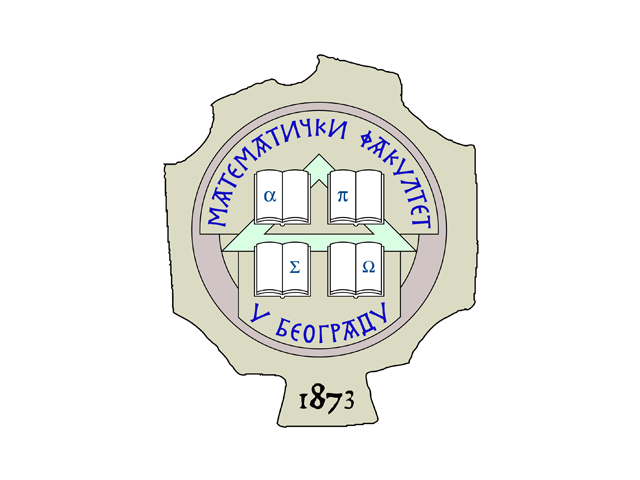
\includegraphics[width=0.4\textwidth]{images/logo.png}
	\end{figure}
    { Univerzitet u Beogradu \\ Matematički fakultet\par}
	
    \vfill

    {\Large \textbf{Seminarski rad}\par}

    \vspace{1cm}

    {\Large \textbf{WAKE WORD DETECTION}\par}

    \vfill

	\begin{tabbing}
	\hspace{10cm} \= \hspace{10cm} \= \kill
	\textbf{Mentor:} \>  \textbf{Studenti:} \\
	Stefan Kapunac \> Iva Milutinović 262/2021 \\
	Katedra za računarstvo i informatiku \> Jovana Medenica 364/2022 \\
	\> Smer: Informatika \\
	\end{tabbing}

    \vfill

    \textbf{Datum:} 2025/26

\end{titlepage}
\newpage

\renewcommand{\contentsname}{Sadržaj}
\renewcommand{\cftsecleader}{\cftdotfill{\cftdotsep}}
\tableofcontents
\newpage

\section{Uvod}


Wake word detection predstavlja problem automatskog prepoznavanja unapred definisane ključne reči ili fraze u audio signalu. Ovakvi sistemi danas imaju veoma široku primenu u savremenim glasovno kontrolisanim uređajima i digitalnim asistentima kao što su Amazon Alexa, Apple Siri i Google Assistant. Njihov osnovni zadatak jeste da kontinuirano analiziraju audio signal i aktiviraju sistem tek nakon detekcije određene ključne reči, čime se omogućava prirodnija i jednostavnija interakcija između čoveka i računara.


Razvoj pouzdanih wake word sistema predstavlja izazovan problem iz oblasti obrade govora i mašinskog učenja. Audio signali mogu sadržati šum, različite akcente, varijacije u brzini govora i različite karakteristike glasa govornika. Pored toga, sistemi za detekciju ključnih reči moraju biti dovoljno precizni da izbegnu lažne aktivacije, ali i dovoljno osetljivi da ne propuste stvarno izgovorenu aktivacionu reč. Zbog toga je izbor odgovarajuće reprezentacije audio signala od velikog značaja za uspešnost sistema.

U sistemima za automatsku obradu govora audio signal se najčešće ne koristi direktno kao ulaz u model mašinskog učenja. Umesto toga, iz audio signala se izdvajaju karakteristične osobine (engl. \textit{features}) koje predstavljaju kompaktniji i informativniji opis govora. Među najpoznatijim metodama za izdvajanje osobina nalaze se Mel-Frequency Cepstral Coefficients (MFCC) i Linear Frequency Cepstral Coefficients (LFCC). MFCC koristi Mel skalu frekvencija koja aproksimira način na koji čovek percipira zvuk, dok LFCC koristi linearno raspoređene frekvencijske filtere i ravnomernije predstavlja čitav frekvencijski opseg audio signala.

U poslednjih nekoliko godina konvolucione neuronske mreže (\textit{Convolutional Neural Networks -- CNN}) pokazale su veoma dobre rezultate u zadacima klasifikacije audio signala i prepoznavanja govora. Razlog tome je činjenica da se reprezentacije poput MFCC i LFCC mogu posmatrati kao dvodimenzionalne matrice slične slikama, što omogućava efikasnu primenu konvolucionih slojeva za prepoznavanje karakterističnih obrazaca u vremensko-frekvencijskom domenu.

U ovom radu razmatra se problem detekcije ključne reči ``stop'' korišćenjem konvolucionih neuronskih mreža. Kao skup podataka korišćen je Google Speech Commands dataset, koji sadrži veliki broj kratkih audio snimaka različitih izgovorenih reči. Poseban fokus rada stavljen je na poređenje dve metode za izdvajanje osobina audio signala -- MFCC i LFCC reprezentacija. Cilj rada nije razvoj nove arhitekture neuronske mreže, već analiza uticaja različitih audio reprezentacija na performanse sistema za wake word detekciju.

U eksperimentalnom delu rada implementiran je jedinstven CNN model koji je treniran odvojeno nad MFCC i LFCC reprezentacijama audio signala. Dobijeni rezultati analizirani su korišćenjem standardnih metrika za klasifikaciju kao što su accuracy, precision, recall i F1-score, sa ciljem određivanja pogodnije reprezentacije za zadatak detekcije ključne reči.


\section{Opis rešenja}

\subsection{Skup podataka}

Za potrebe razvoja i testiranja sistema za detekciju ključne reči korišćen je Google Speech Commands dataset. Ovaj skup podataka predstavlja jedan od najčešće korišćenih skupova podataka u zadacima prepoznavanja govora i klasifikacije kratkih audio komandi. Dataset sadrži veliki broj audio snimaka različitih reči izgovorenih od strane velikog broja govornika različitog pola, uzrasta i akcenata.

Audio snimci u dataset-u sačuvani su u \texttt{.wav} formatu, pri čemu svaki snimak traje približno jednu sekundu. Uzorci su snimani sa frekvencijom od 16 kHz i predstavljaju kratke govorne komande poput \textit{stop}, \textit{go}, \textit{left}, \textit{right}, \textit{yes}, \textit{no} i druge.

U okviru ovog rada kao aktivaciona reč (\textit{wake word}) odabrana je reč \textit{``stop''}. Problem je formulisan kao zadatak binarne klasifikacije:
\begin{itemize}
    \item pozitivna klasa predstavlja audio snimke reči \textit{``stop''},
    \item negativna klasa obuhvata sve ostale reči iz dataset-a.
\end{itemize}

Na ovaj način model uči da razlikuje ciljnu ključnu reč od ostalih govornih komandi. Za svaki audio snimak vršeno je izdvajanje karakterističnih osobina audio signala korišćenjem MFCC i LFCC reprezentacija, koje su zatim korišćene kao ulaz u konvolucionu neuronsku mrežu.

Na slici \ref{fig:waveform_stop} prikazan je primer audio signala reči \textit{``stop''} iz korišćenog skupa podataka.

\begin{figure}[H]
    \centering
    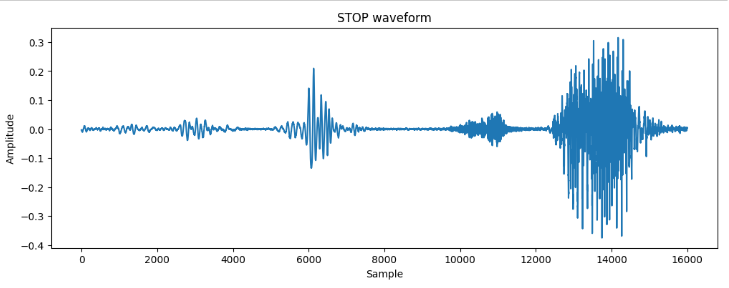
\includegraphics[width=0.9\textwidth]{images/stop_waveform.png}
    \caption{Prikaz audio signala reči ``stop'' iz Google Speech Commands dataset-a}
    \label{fig:waveform_stop}
\end{figure}

\subsection{Pretprocesiranje audio signala}

Pre izdvajanja karakterističnih osobina audio signala bilo je potrebno izvršiti pretprocesiranje audio podataka kako bi svi ulazni primeri imali uniforman format pogodan za obradu neuronskom mrežom. Pretprocesiranje predstavlja važan korak u sistemima za obradu govora, jer omogućava stabilnije i efikasnije treniranje modela.

Audio snimci iz Google Speech Commands dataset-a učitavani su korišćenjem biblioteke \texttt{Librosa}. Svi audio fajlovi konvertovani su na frekvenciju od 16 kHz, što predstavlja standardnu frekvenciju uzorkovanja u zadacima prepoznavanja govora. Nakon učitavanja audio signal je podeljen na manje vremenske segmente korišćenjem Short-Time Fourier Transform (STFT) metode, čime je omogućena analiza frekvencijskih karakteristika zvuka kroz vreme.

Nakon transformacije audio signala u vremensko-frekvencijski domen vršeno je izdvajanje karakterističnih osobina korišćenjem MFCC i LFCC reprezentacija. Ove reprezentacije omogućavaju kompaktniji opis audio signala i isticanje informacija relevantnih za razlikovanje govornih komandi.

Dobijene MFCC i LFCC matrice nisu imale identične dimenzije za sve audio snimke, zbog čega je bilo potrebno izvršiti usklađivanje dimenzija. U okviru implementacije korišćen je postupak \textit{padding/truncation}, pri čemu su kraće matrice dopunjavane nulama, dok su duže matrice skraćivane na unapred definisanu maksimalnu dužinu. Na taj način svi ulazni primeri dobili su jedinstvenu dimenziju pogodnu za ulaz u konvolucionu neuronsku mrežu.

Nakon formiranja konačnog skupa podataka izvršena je podela na trening i test skup korišćenjem funkcije \texttt{train\_test\_split} iz biblioteke \texttt{Scikit-learn}. Za treniranje modela korišćeno je 75\% podataka, dok je preostalih 25\% korišćeno za evaluaciju uspešnosti modela. Podela je izvršena uz očuvanje odnosa klasa korišćenjem \textit{stratified split} pristupa.

Kompletan postupak pretprocesiranja audio signala prikazan je na slici \ref{fig:pipeline}.

\begin{figure}[!ht]
    \centering
    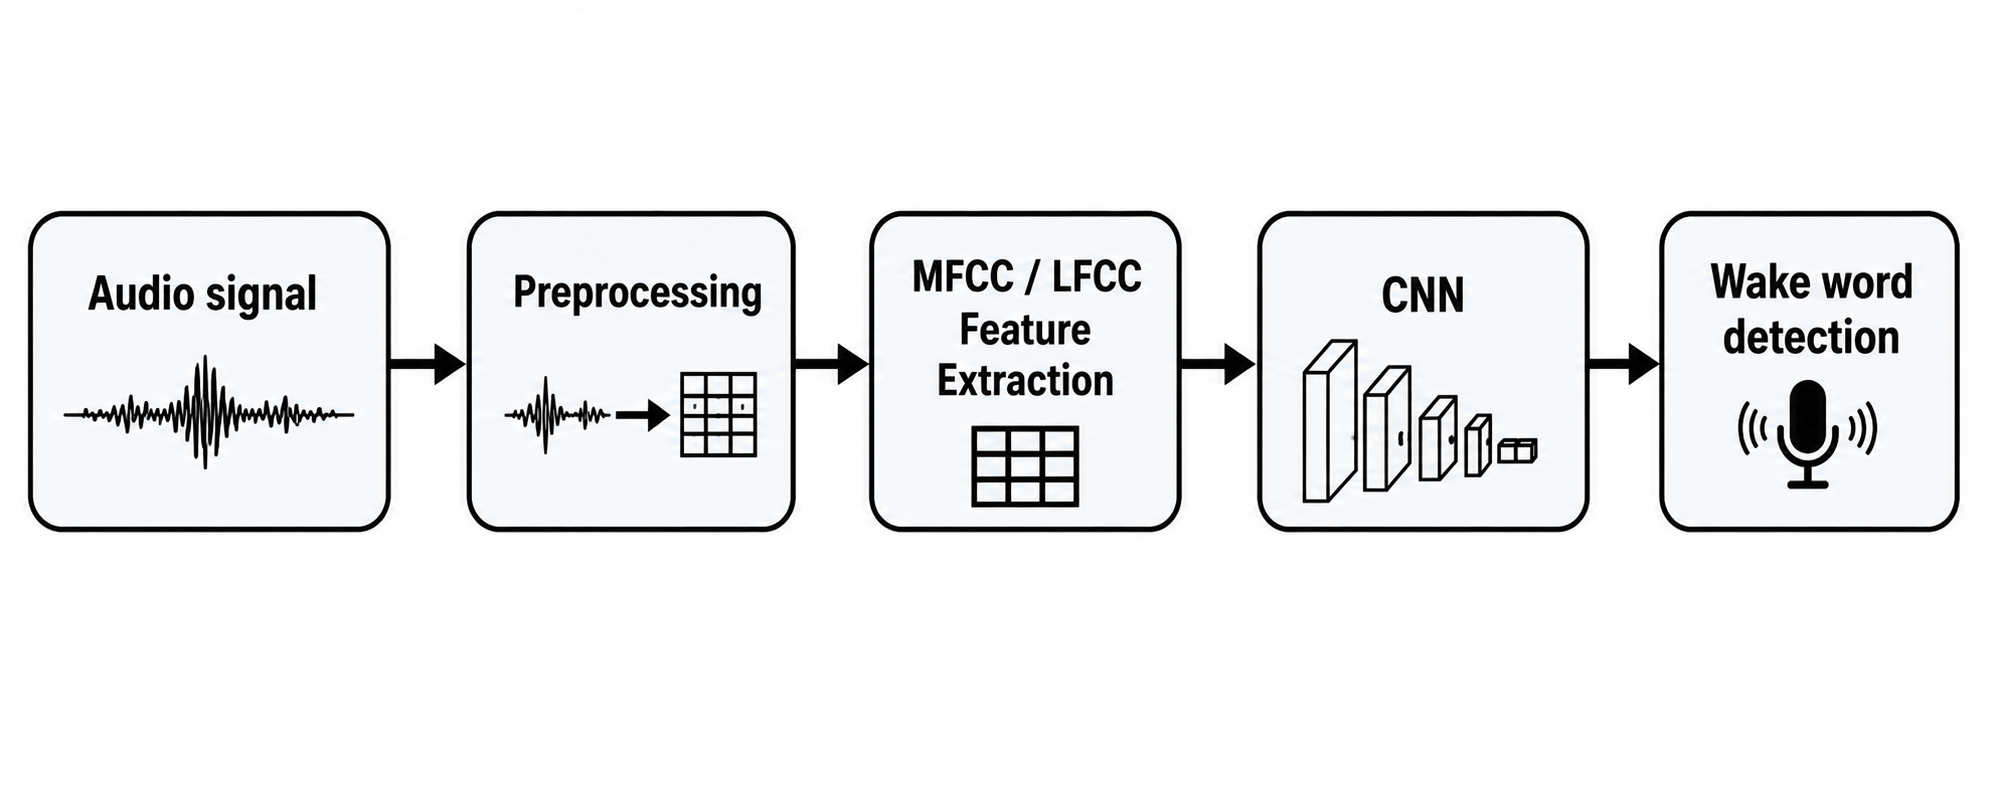
\includegraphics[width=0.9\textwidth]{images/pipeline.png}
    \caption{Pipeline sistema za wake word detekciju}
    \label{fig:pipeline}
\end{figure}

\subsection{MFCC reprezentacija}

\subsection{LFCC reprezentacija}

Linear Frequency Cepstral Coefficients (LFCC) predstavljaju jednu od metoda za izdvajanje karakterističnih osobina audio signala koja se često koristi u zadacima obrade govora i audio klasifikacije. LFCC reprezentacija omogućava transformaciju audio signala iz vremenskog domena u kompaktnu vremensko-frekvencijsku reprezentaciju pogodnu za obradu metodama mašinskog učenja.

Za razliku od MFCC reprezentacije, koja koristi Mel skalu frekvencija zasnovanu na načinu na koji čovek percipira zvuk, LFCC koristi linearno raspoređene frekvencijske filtere. Na ovaj način čitav frekvencijski opseg audio signala tretira se ravnomerno, bez dodatnog naglašavanja nižih frekvencija. Zbog toga LFCC reprezentacija može sačuvati više informacija o višim frekvencijama audio signala.

Proces izdvajanja LFCC karakteristika započinje podelom audio signala na manje vremenske segmente. Nakon toga nad svakim segmentom primenjuje se Short-Time Fourier Transform (STFT), čime se audio signal transformiše iz vremenskog u frekvencijski domen. Dobijeni spektrogram zatim prolazi kroz skup linearno raspoređenih frekvencijskih filtera (\textit{linear filter bank}), koji mere energiju signala u različitim frekvencijskim opsezima.

Nakon filtriranja primenjuje se logaritamska transformacija radi smanjenja dinamičkog opsega vrednosti i stabilizacije reprezentacije audio signala. Na kraju se primenjuje Discrete Cosine Transform (DCT), čime se dobijaju cepstralni koeficijenti koji predstavljaju konačnu LFCC reprezentaciju audio signala.

Kompletan postupak izdvajanja LFCC karakteristika prikazan je na slici \ref{fig:lfcc_pipeline}.

\begin{figure}[H]
    \centering
    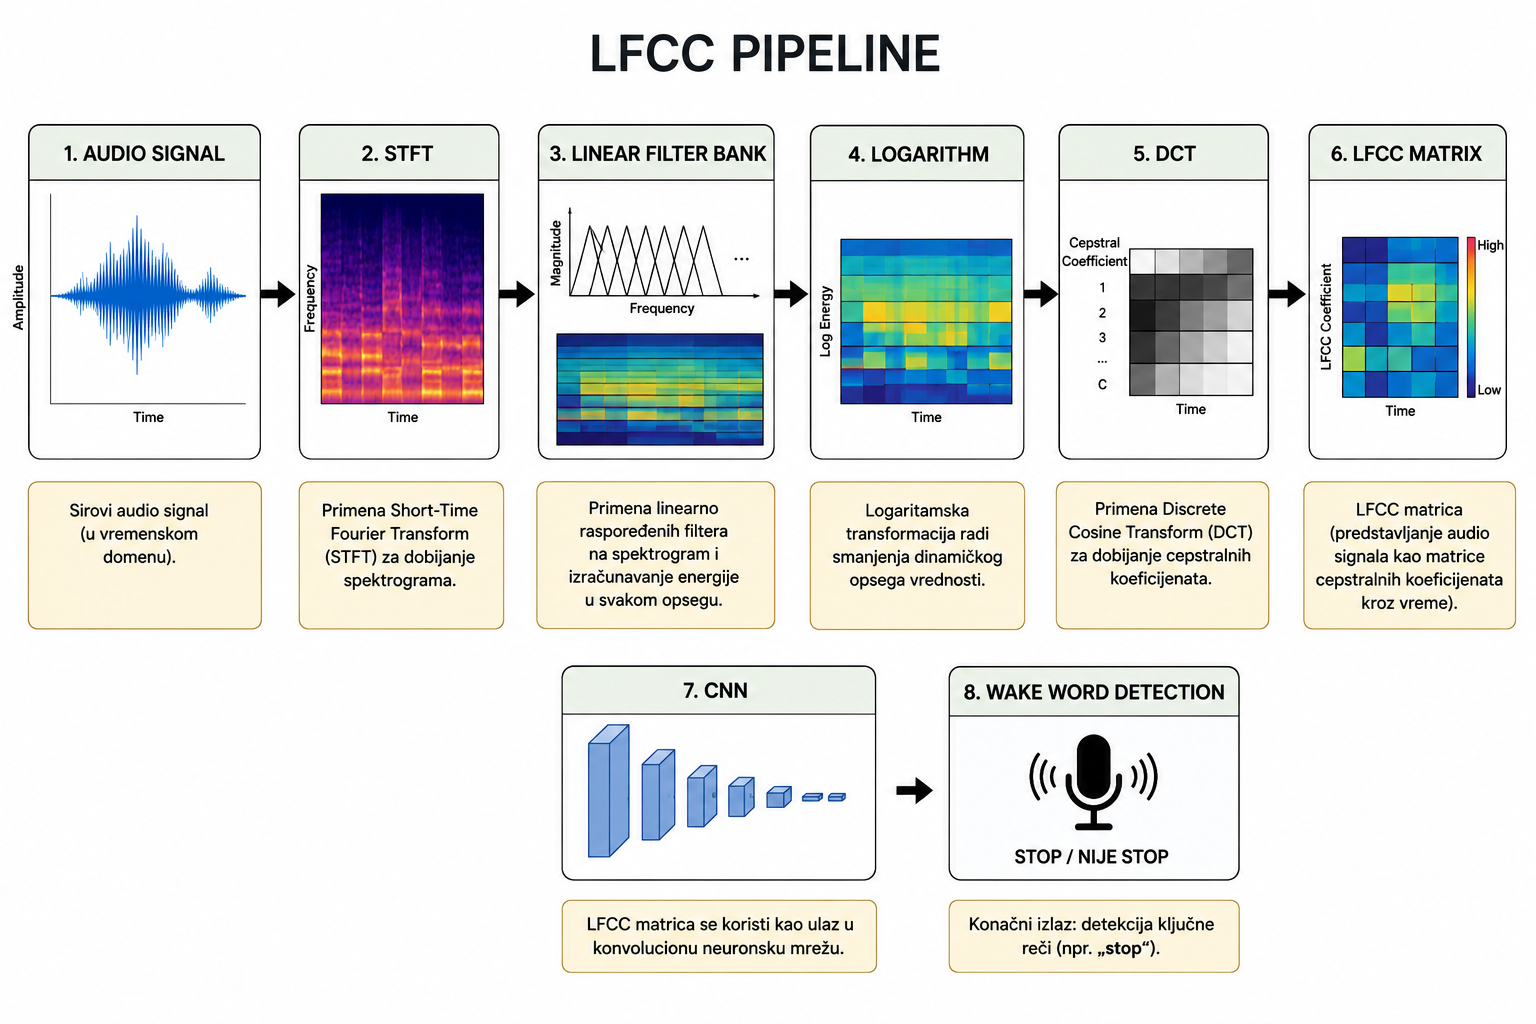
\includegraphics[width=0.9\textwidth]{images/lfcc_pipeline.png}
    \caption{Postupak izdvajanja LFCC karakteristika}
    \label{fig:lfcc_pipeline}
\end{figure}

LFCC matrica predstavlja vremensko-frekvencijsku reprezentaciju audio signala, pri čemu redovi matrice predstavljaju cepstralne koeficijente, dok kolone predstavljaju vremenske segmente audio signala. Na ovaj način moguće je analizirati promene frekvencijskih karakteristika govora kroz vreme.

U okviru implementacije za svaki vremenski segment audio signala računato je 13 LFCC koeficijenata. Audio signal je podeljen na 32 vremenska segmenta, zbog čega konačna LFCC reprezentacija ima dimenzije 13×32. Kako bi svi ulazni primeri imali iste dimenzije pogodne za obradu konvolucionom neuronskom mrežom, primenjen je postupak dopunjavanja ili skraćivanja matrica (\textit{padding/truncation}).

Primer LFCC matrice za audio signal reči ``stop'' prikazan je na slici \ref{fig:lfcc_matrix}.

\begin{figure}[!ht]
    \centering
    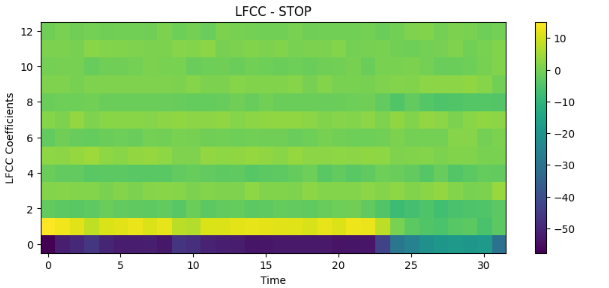
\includegraphics[width=0.8\textwidth]{images/lfcc_matrix.png}
    \caption{LFCC matrica za audio signal reči ``stop''}
    \label{fig:lfcc_matrix}
\end{figure}

Sa slike \ref{fig:lfcc_matrix} može se uočiti vremensko-frekvencijska reprezentacija audio signala reči ``stop'' dobijena korišćenjem LFCC metode. Horizontalna osa predstavlja vremenske segmente audio signala, dok vertikalna osa predstavlja LFCC koeficijente.

Različite boje u matrici predstavljaju različite vrednosti energije u određenim frekvencijskim opsezima. Svetlije oblasti označavaju veće vrednosti koeficijenata, dok tamnije oblasti predstavljaju manje vrednosti energije signala.

Može se primetiti da se tokom izgovora reči ``stop'' određeni LFCC koeficijenti značajno menjaju kroz vreme, što ukazuje na promenu frekvencijskih karakteristika govora. Posebno su izražene promene u nižim koeficijentima, koji sadrže najvažnije informacije o spektralnoj strukturi audio signala.

LFCC matrica predstavlja kompaktan opis audio signala i omogućava konvolucionoj neuronskoj mreži da efikasno prepoznaje karakteristične obrasce povezane sa izgovorom ključne reči.



\subsection{CNN arhitektura}

Za klasifikaciju audio signala i detekciju ključne reči korišćena je konvoluciona neuronska mreža (Convolutional Neural Network -- CNN). Konvolucione neuronske mreže pokazale su veoma dobre rezultate u zadacima klasifikacije slika, obrade zvuka i prepoznavanja govora zbog sposobnosti automatskog izdvajanja karakterističnih obrazaca iz ulaznih podataka.

U ovom radu LFCC matrice korišćene su kao ulaz u CNN model. Pošto LFCC reprezentacija ima oblik dvodimenzione matrice, moguće ju je posmatrati na sličan način kao sliku, što omogućava efikasnu primenu konvolucionih slojeva za prepoznavanje lokalnih vremensko-frekvencijskih obrazaca u audio signalu.

Korišćena CNN arhitektura sastoji se iz dva konvoluciona sloja, pooling slojeva i potpuno povezanih (\textit{fully connected}) slojeva. Prvi konvolucioni sloj koristi 16 filtera dimenzije \(3 \times 3\), dok drugi konvolucioni sloj koristi 32 filtera iste dimenzije. Nakon svakog konvolucionog sloja primenjuje se ReLU aktivaciona funkcija, koja uvodi nelinearnost u model i omogućava učenje složenijih obrazaca.

Radi smanjenja dimenzionalnosti podataka i smanjenja mogućnosti preprilagođavanja modela korišćen je MaxPooling sloj dimenzije \(2 \times 2\). Nakon konvolucionih slojeva i pooling operacija izlaz se transformiše u jednodimenzioni vektor koji se prosleđuje potpuno povezanim slojevima.

Prvi potpuno povezani sloj sadrži 64 neurona i koristi ReLU aktivacionu funkciju, dok završni sloj sadrži jedan neuron sa sigmoid aktivacionom funkcijom. Sigmoid funkcija vraća vrednost u opsegu od 0 do 1 i predstavlja verovatnoću da audio signal sadrži ključnu reč ``stop''.

Arhitektura korišćene konvolucione neuronske mreže prikazana je na slici \ref{fig:cnn_architecture}.

\begin{figure}[H]
    \centering
    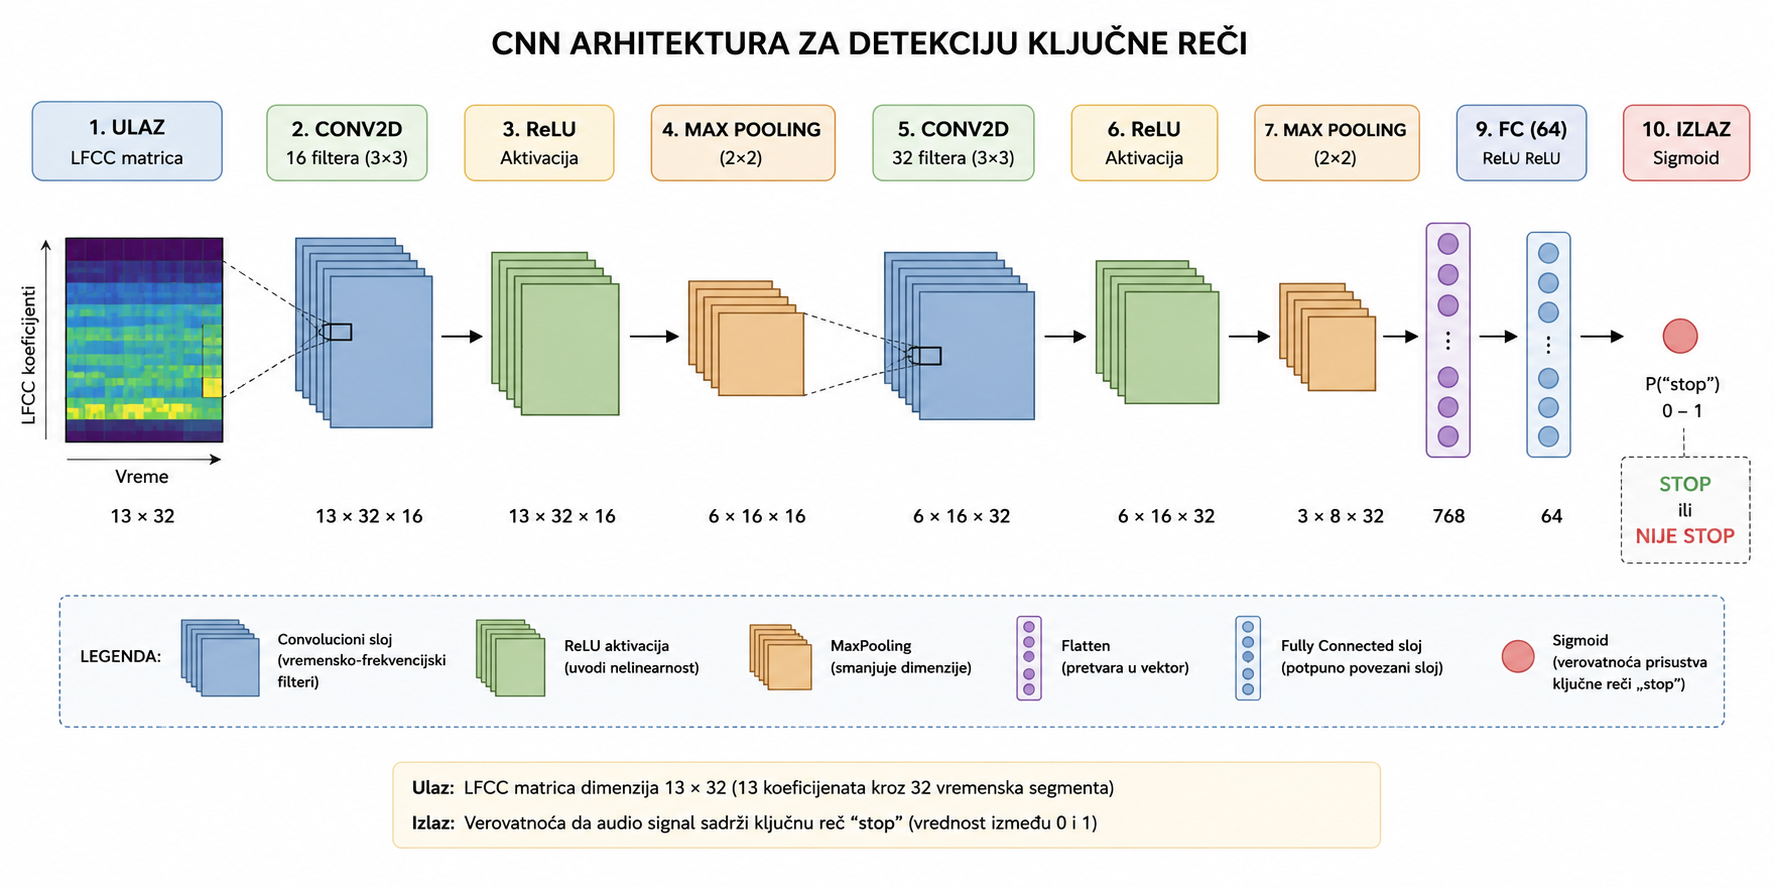
\includegraphics[width=0.9\textwidth]{images/cnn_architecture.png}
    \caption{Arhitektura konvolucione neuronske mreže korišćene za detekciju ključne reči}
    \label{fig:cnn_architecture}
\end{figure}

\subsection{Treniranje modela}

Nakon formiranja LFCC reprezentacija i definisanja arhitekture konvolucione neuronske mreže izvršeno je treniranje modela za zadatak detekcije ključne reči. Skup podataka podeljen je na trening i test skup korišćenjem funkcije \texttt{train\_test\_split} iz biblioteke \texttt{Scikit-learn}. Za treniranje modela korišćeno je 75\% podataka, dok je preostalih 25\% korišćeno za evaluaciju uspešnosti modela. Podela podataka izvršena je korišćenjem stratifikovanog pristupa kako bi odnos pozitivne i negativne klase bio očuvan u oba skupa.

Pre početka treniranja podaci su konvertovani u PyTorch tenzore i prilagođeni formatu pogodnom za ulaz u konvolucionu neuronsku mrežu. LFCC matrice proširene su dodatnom dimenzijom kanala kako bi odgovarale očekivanom formatu ulaza oblika \(batch\_size \times channels \times height \times width\).

Za treniranje modela korišćena je Binary Cross-Entropy (BCE) funkcija gubitka, pogodna za probleme binarne klasifikacije. Kao optimizer korišćen je Adam optimizer sa stopom učenja od 0.001. Treniranje modela vršeno je u mini-batchevima veličine 32 uzorka tokom 10 epoha.

Tokom procesa treniranja za svaki batch vršeno je prosleđivanje podataka kroz mrežu (\textit{forward propagation}), računanje funkcije gubitka, a zatim ažuriranje parametara mreže korišćenjem postupka propagacije greške unazad (\textit{backpropagation}). Cilj treniranja bio je minimizacija funkcije gubitka i poboljšanje sposobnosti modela da razlikuje prisustvo i odsustvo ključne reči ``stop''.

Implementacija modela realizovana je korišćenjem Python programskog jezika i PyTorch biblioteke za razvoj neuronskih mreža.

\begin{figure}[H]
    \centering
    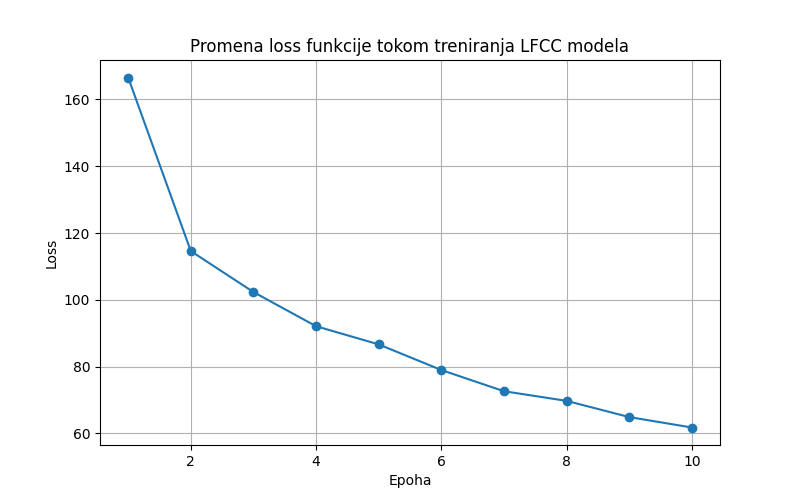
\includegraphics[width=0.75\textwidth]{images/lfcc_loss.png}
    \caption{Promena vrednosti funkcije gubitka tokom treniranja LFCC modela}
    \label{fig:lfcc_loss}
\end{figure}

Sa slike \ref{fig:lfcc_loss} može se primetiti da vrednost funkcije gubitka postepeno opada tokom epoha, što ukazuje na uspešno treniranje modela i prilagođavanje parametara mreže zadatom problemu klasifikacije.

\section{Eksperimentalni rezultati} 

\subsection{Rezultati MFCC modela} 

\subsection{Rezultati LFCC modela}

Nakon treniranja CNN modela nad LFCC reprezentacijama izvršena je evaluacija uspešnosti modela na test skupu podataka. Evaluacija je sprovedena korišćenjem metrika accuracy, precision, recall i F1-score, kao i analizom konfuzione matrice.

LFCC model ostvario je tačnost klasifikacije od 98.50\% na test skupu, što ukazuje na veoma uspešno razlikovanje prisustva i odsustva ključne reči ``stop''.

Dobijena konfuziona matrica prikazana je na slici \ref{fig:lfcc_cm}. Iz matrice se može primetiti da model veoma uspešno prepoznaje negativnu klasu, dok se određeni broj grešaka javlja kod detekcije pozitivne klase.

\begin{figure}[H]
    \centering
    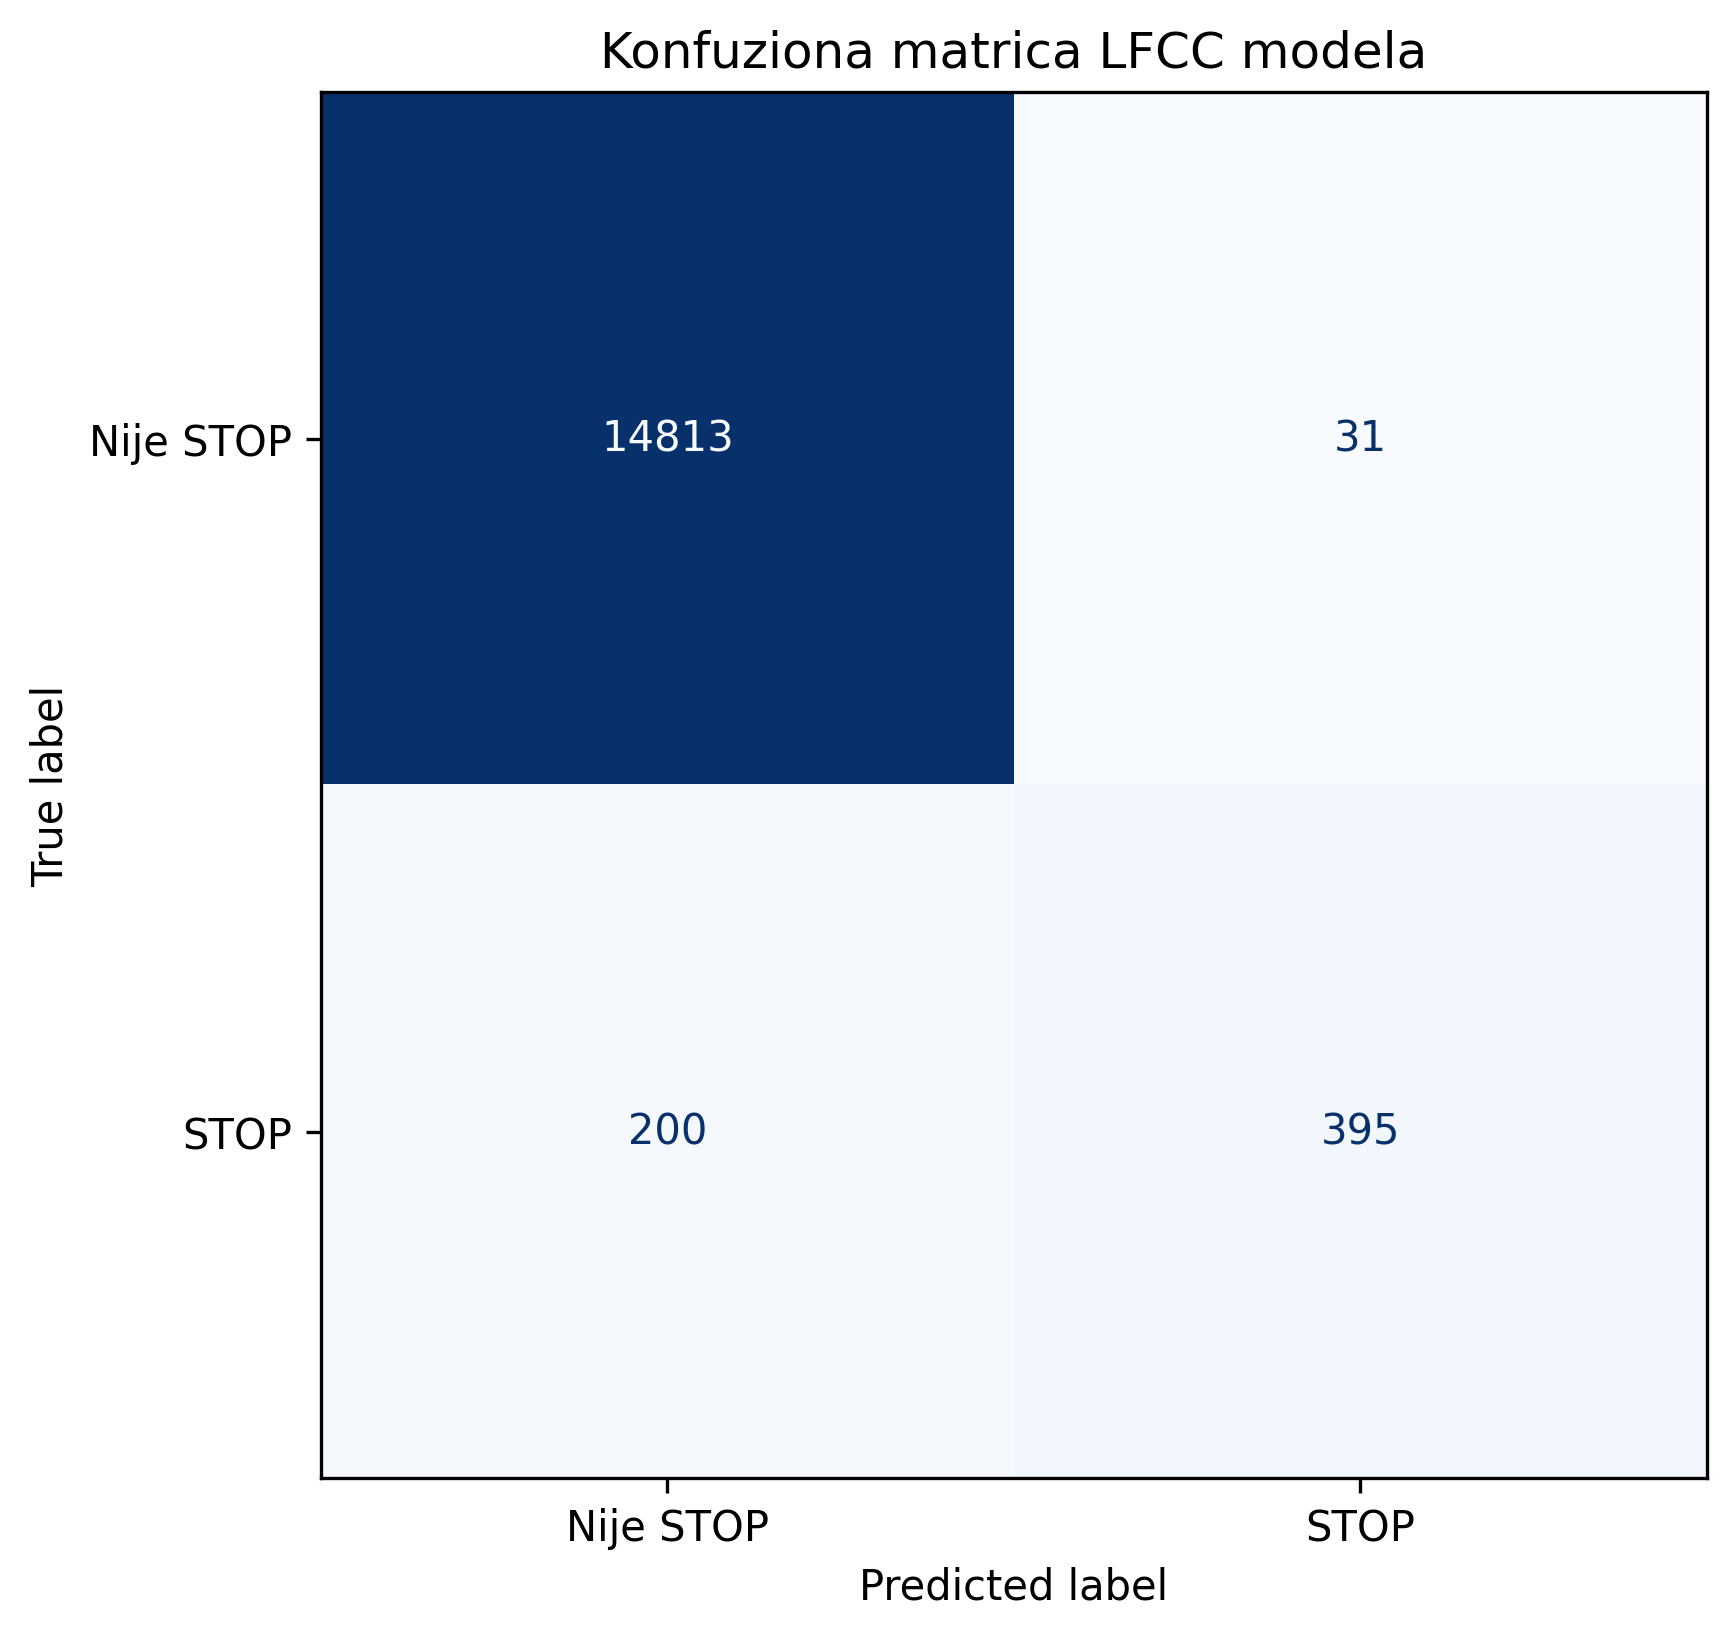
\includegraphics[width=0.6\textwidth]{images/lfcc_confusion_matrix.png}
    \caption{Konfuziona matrica LFCC modela}
    \label{fig:lfcc_cm}
\end{figure}

Na slici \ref{fig:lfcc_report} prikazan je detaljan izveštaj klasifikacije modela. Model ostvaruje precision vrednost od 0.93 za pozitivnu klasu, što znači da je broj lažno pozitivnih detekcija relativno mali. Drugim rečima, kada model predvidi prisustvo ključne reči ``stop'', ta predikcija je u velikom broju slučajeva tačna.

Sa druge strane, recall vrednost iznosi 0.66, što ukazuje da model ne prepoznaje sve stvarne primere ključne reči i da određeni broj pozitivnih uzoraka ostaje neotkriven. Ovakav rezultat može biti posledica varijacija u izgovoru, prisustva šuma u audio signalima, različite jačine govora ili neuravnoteženosti skupa podataka, s obzirom da negativna klasa sadrži značajno više uzoraka od pozitivne klase.

F1-score za pozitivnu klasu iznosi 0.77 i predstavlja kompromis između precision i recall metrike. Dobijena vrednost ukazuje da model ostvaruje stabilne performanse, ali da postoji prostor za dodatno unapređenje detekcije aktivacione reči.

Recall vrednost mogla bi biti poboljšana korišćenjem većeg broja pozitivnih uzoraka, primenom tehnika augmentacije audio signala, balansiranjem klasa ili treniranjem kompleksnijih modela sa većim brojem epoha i slojeva. Takođe, dodatno podešavanje hiperparametara moglo bi doprineti boljoj sposobnosti modela da prepozna različite varijacije ključne reči ``stop''.
\begin{figure}[H]
    \centering
    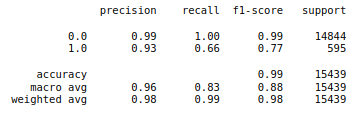
\includegraphics[width=0.7\textwidth]{images/lfcc_classification_report.png}
    \caption{Classification report LFCC modela}
    \label{fig:lfcc_report}
\end{figure}


\subsection{Poređenje MFCC i LFCC pristupa} 

\subsection{Diskusija rezultata}

\section{Zaključak} 


\end{document}
